\section{Przypadek Testowy 1- Najbliższy sąsiad, a rozszerzony najbliższy sąsiad- porównanie wyników oraz czasów wykonywania}
  \subsection{Cel:}
    W tej części zostaną ze sobą porównanie dwie bardzo podobne metody rozwiązywania problemu komiwojażera- algorytm najbliższego sąsiada oraz rozszerzony algorytm najbliższego sąsiada. Ze względu na to, iż w rozszerzonym sąsiedzie aby oduzależnić otrzymany wynik od wierzchołka początkowego, przechodzimy po wszystkich wierzchołkach, naturalnym jest, iż spodziewamy się otrzymywać lepszy wynik w nieco dłuższym czasie. Celem tego testu będzie zbadanie, czy w każdym przypadku stosowanie rozszerzonego algorytmu najbliższego sąsiada jest zdecydowanie lepsze od swojego poprzednika. 
  \subsection{Założenia:}
    Do tego badania użyto automatycznie wygenerowanych grafów typu \textbf{EUC2D}. Rozmiary grafów (oznaczane literą n) należą do zbioru $n \in \{10,15,20,...,100\}$. Dla algorytmu najbliższego sąsiada dla zadanej długości grafu badanie powtórzono 5 razy.

  \subsection{Wyniki: }
    Poniższa tabele przedstawiają wyniki wykonanych testów:
    \begin{table}[H]
    \begin{tabular}{|c | c | c |} 
     \hline
     n & Najbliższy & Rozszerzony \\ [0.5ex] 
     \hline\hline
      10  & 9,786950732 &0 \\
      15  & 7,120743034 &0 \\
      20  & 11,19483315 &6,779661017 \\
      25  & 15,79634465 &5,147058824 \\
      30  & 12,10191083 &1,193317422 \\
      35  & 11,13360324 &1,126126126 \\
      40  & 13,58260206 &1,091703057 \\
      45  & 16,03927987 &4,469273743 \\
      50  & 23,79562044 &4,744525547 \\
      55  & 16,00127755 &8,202443281 \\
      60  & 34,19556566 &26,15629984 \\
      65  & 23,64657814 &10,74626866 \\
      70  & 17,08344301 &9,612625538 \\ 
      75  & 12,67305644 &5,747126437 \\
      80  & 18,91247317 &9,574468085 \\
      85  & 21,60317111 &11,11111111 \\
      90  & 20,33256157 &9,341317365 \\
      95  & 23,46057932 &15,91148577 \\
      100 & 21,46546776 &6,385404789 \\
     \hline
    \end{tabular}
    \caption{Współczynnik PRD dla otrzymanych wyników. Za wartość referencyjną posłużył wynik otrzymany przez algorytm 2-opt z elementem startowym wyznaczonym przez najbliższego sasiada}
    \end{table}

    \begin{table}[H]
    \begin{tabular}{|c | c | c | c | c |} 
     \hline
     n & DrogaNajbliższy & CzasNajbliższy & DrogaRozszerzony & CzasRozszerzony \\ [0.5ex] 
     \hline\hline
      10  & 300,4 & 0,192 & 271 & 1,97 \\
      15  & 323 & 0,41 &  300 & 1,95 \\
      20  & 371,6 & 0,646 &  354 & 125,88 \\
      25  & 459,6 & 0,996 & 408 & 23,74 \\
      30  & 471 & 1,4 & 419 & 39,84 \\
      35  & 494 &  1,838 & 444 & 64,69 \\
      40  & 524,2 & 2,372 & 458 & 98,93 \\
      45  & 611 & 3,004 & 537 &  145,38 \\
      50  & 685 & 3,998 & 548 &  180,72 \\
      55  & 626,2 & 4,782 & 573 & 249,38 \\ 
      60  & 703,6 & 5,494 & 627 & 313,86 \\
      65  & 783,2 & 6,778 & 670 & 394,06 \\
      70  & 759,8 & 7,352 & 697 & 496,95 \\
      75  & 751,2 & 8,576 & 696 & 496,95 \\
      80  & 838,6 & 9,606 & 752 & 611,32 \\
      85  & 908,2 & 11,43 & 801 & 864,69 \\
      90  & 950,2 & 11,932  & 835 & 1042,41 \\
      95  & 1042,6  & 13,768  & 949 & 1244,87 \\
      100 & 1045,4  & 14,204  & 877 & 1430,27 \\

     \hline
    \end{tabular}
    \caption{Wyniki dróg i czasów dla rozpatrywanych wariantów (należy pamiętać, że dla algorytmu najbliższego sąsiada są to wartości \textbf{uśrednione!}. Jednostką czasu są milisekundy)}
    \end{table}

  \subsection{Wykresy: }
    \begin{figure}[H]
      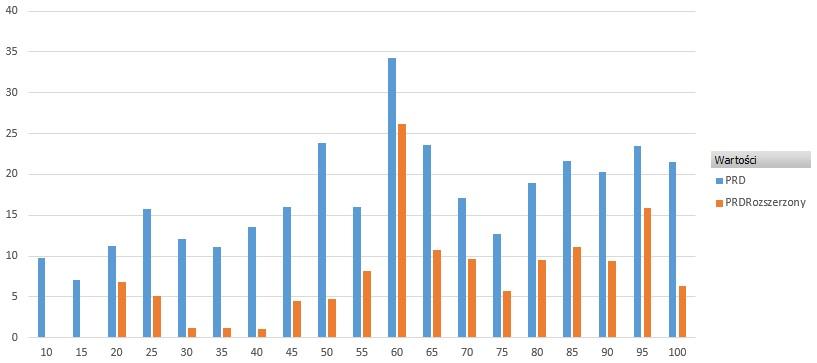
\includegraphics[scale=0.75]{prd}
      \centering
      \caption{Współczynnik PRD dla testowanych algorytmów}
    \end{figure}
    \begin{figure}[H]
      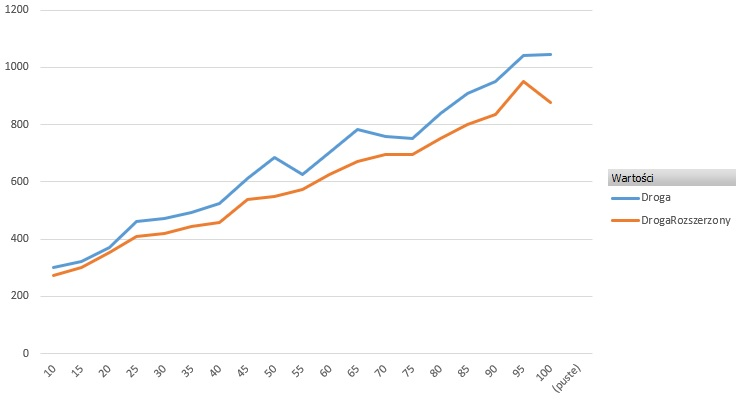
\includegraphics[scale=0.8]{zaleznoscDrogi}
      \centering
      \caption{Osiagniete minimalne funkcje celu dla testowanych algorytmów}
    \end{figure}

  \subsection{Wnioski: }
    Zauważamy, iz mimo otrzymywania lepszych wyników dla rozszerzonego algorytmu najbliższego sąsiada, czasy, w jakich je otrzymujemy są zdecydowanie gorsze niż dla najbliższego sąsiada dla losowo wybranego elementu początkowego. Dodatkowo różnice w otrzymanych drogach są niewielkie, co powoduje, iż nie zawsze korzystanie z algorytmu rozszerzonego sąsiada jest optymalne. Należy dodatkowo zauważyc, iż na różnice czasowe mogą wpływać takie aspekty jak: sprzęt, na którym wykonywano testy oraz język programowania, w którym ów test został wykonany.

